\documentclass[xcolor=dvipsnames]{beamer}
\usepackage[english]{babel}
\usepackage[latin1]{inputenc}
\usepackage{times}
\usepackage[T1]{fontenc}
\usepackage{graphicx}
\usepackage[absolute, overlay]{textpos}
\usepackage{tikz}
\usepackage{multimedia}
\usepackage{soul}
\usepackage{wasysym}
\def\urltilda{\kern -.15em\lower .7ex\hbox{\~{}}\kern .04em}
\def\deg{^{\circ}}

\setlength{\TPHorizModule}{0.01\textwidth}
\setlength{\TPVertModule}{\TPHorizModule}
\definecolor{darkyellow}{rgb}{1,0.75,0}
\definecolor{black}{rgb}{0,0,0}
\definecolor{skyblue}{rgb}{0.7,0.8,1.0}
\definecolor{black}{rgb}{0,0,0}
\definecolor{darkgrey}{rgb}{0.3,0.3,0.3}
\definecolor{medgrey}{rgb}{0.5,0.5,0.5}
\definecolor{lightgrey}{rgb}{0.8,0.8,0.8}
\definecolor{lightMahogany}{rgb}{0.9,0.8,0.8}
\definecolor{darkblue}{rgb}{0,0,0.5}
\definecolor{darkgreen}{rgb}{0.1,0,0.3}
\definecolor{darkred}{rgb}{0.6,0,0}

\newcommand{\params}{\Xi}
\newcommand{\Eobsi}{E'_i}
\newcommand{\phiobsi}{\phi'_i}
\newcommand{\Etruei}{E_i}
\newcommand{\phitruei}{\phi_{i}}
\newcommand{\Eobsij}{E'_{ij}}
\newcommand{\phiobsij}{\phi'_{ij}}
\newcommand{\Etrueij}{E_{ij}}
\newcommand{\phitrueij}{\phi_{ij}}
\newcommand{\obs}{\mathrm{obs}}
\newcommand{\true}{\mathrm{true}}
\newcommand{\Like}{\mathcal{L}}
\newcommand{\ntot}{{n_\mathrm{tot}}}
\newcommand{\ntotj}{{n_{\mathrm{tot},j}}}
\newcommand{\diff}{\mathrm{d}}
\newcommand{\cblue}[1]{{\color[rgb]{0.1, 0.0, 0.6} #1}}
\newcommand{\cgreen}[1]{{\color[rgb]{0.0, 0.6, 0.1} #1}}
\newcommand{\corange}[1]{{\color[rgb]{0.9, 0.5, 0.0} #1}}
\newcommand{\cbluewhen}[2]{{\color#2[rgb]{0.1, 0.0, 0.6} #1}}
\newcommand{\cgreenwhen}[2]{{\color#2[rgb]{0.0, 0.6, 0.1} #1}}
\newcommand{\corangewhen}[2]{{\color#2[rgb]{0.9, 0.5, 0.0} #1}}

\newcommand{\manual}[1]{
  \begin{tikzpicture}[x=\textwidth, y=0.82\textheight]%, >=angle 90]
    \useasboundingbox (0, 0) rectangle (1, 1);
    #1
  \end{tikzpicture}
}

%%% Custom nodes.

\newcommand{\basenode}[4]{
  \node[outer sep=6pt, anchor=#3] (#1) at (#2){#4};
}

\newcommand{\emptynode}[2]{
  \basenode{#1}{#2}{base}{}

}

\newcommand{\minipagenode}[5]{
  \basenode{#1}{#2}{#3}{
    \begin{minipage}{#4}
      \vspace*{-12pt}
      {#5}
      \vspace*{-8pt}
  \end{minipage}}

}

\newcommand{\imagenode}[5]{
  \minipagenode{#1}{#2}{#3}{#4}{%
    \includegraphics[width=\textwidth]{#5}%
  }
}

%%% Connectors.

\newcommand{\connect}[4]{%
  \draw[<->, color=darkpurple, line width=1pt, out=#3, in=#4] (#1) to (#2);
}
\newcommand{\connectcolor}[5]{%
  \draw[<->, color=#5, line width=1pt, out=#3, in=#4] (#1) to (#2);
}
\newcommand{\hconnect}[3]{%
  \draw[<->, color=darkpurple, line width=1pt]
  (#1.east) .. controls +(right:#3) and +(left:#3) .. (#2.west);
}
\newcommand{\vconnect}[3]{%
  \draw[<->, color=darkpurple, line width=1pt]
  (#1.south) .. controls +(down:#3) and +(up:#3) .. (#2.north);
}

\newenvironment{litemize}
{\usebeamercolor[fg]{item color}%
\scriptsize\begin{list}{$\bullet$}{%
\setlength{\itemindent}{0pt}%
\setlength{\labelwidth}{10pt}%
\setlength{\leftmargin}{15pt}%
}}
{\end{list}}

\mode<presentation>
{
  \usetheme{Warsaw}
  \usecolortheme[named=Mahogany]{structure}
  \setbeamercovered{transparent}
  \setbeamercolor*{section in toc}{bg=white, fg=Mahogany}
}

%\beamerdefaultoverlayspecification{<+->}

\AtBeginSubsection[]
{
  \begin{frame}<beamer>
    \frametitle{Outline}
  \begin{columns}[t]
\column{0.8\textwidth}
\tableofcontents[sections={1-3}, currentsection, currentsubsection]
  \end{columns}
  \end{frame}
}

\setbeamertemplate{subsection in head/foot shaded}
{\textcolor{structure!70!white}{\insertsubsectionhead}}
\setbeamertemplate{subsection in head/foot}{\textcolor{white}\insertsubsectionhead}

\title[{\textcolor{white}Statistical challenges in astroparticle physics}]{\textcolor{white}{Statistical challenges in astroparticle physics}}
\author[\textcolor{medgrey}{Pat Scott -- Mar 20 -- CosmoStats13, Banff}]{Pat Scott}
\institute{\small{Department of Physics, McGill University}}
\date[Mar 20 2013]{Slides available from \color[rgb]{0.1, 0.2, 0.6} \href{http://www.physics.mcgill.ca/~patscott}{\tt http://www.physics.mcgill.ca/{\urltilda}patscott}}
\pgfdeclareimage[height=0.7cm]{university-logo}{McGill_crest}
\logo{\pgfuseimage{university-logo}}

\subject{Talks}

\begin{document}

\begin{frame}
  \titlepage
\end{frame}

\begin{frame}<beamer>
  \frametitle{Outline}
\begin{columns}[t]
  \column{0.8\textwidth}
  \tableofcontents[sections={1-3}]
\end{columns}
\end{frame}

\section{Overview}

\begin{frame}
\frametitle{My view of astroparticle physics}

How to define astroparticle physics?\vspace{3mm}

\visible<2->{

\begin{columns}[t]
\column{0.5\textwidth}
\uncover<1-3>{%
\footnotesize
\textbf{Option A}\\
Use of known \cblue{particle physics} to tell us something about \cblue{astronomical objects/processes}
\begin{itemize}
  \item Cosmic rays
  \item Supernova interiors, remnants
  \item Blazar, pulsar/magnetar studies
  \item Gravitational wave astronomy
\end{itemize}
}

\column{0.5\textwidth}
\footnotesize
\visible<3->{%
\textbf{Option B}\\
Use of \cblue{astronomical probes} to tell us new things about \cblue{particle/fundamental physics}
\begin{itemize}
  \item Dark matter searches
  \item Cosmological neutrino probes
  \item Big Bang Nucleosynthesis
  \item Inflationary theory testing
\end{itemize}

}

\end{columns}\vspace{4mm}

\visible<4->{
Both are legitimate -- \alert<4->{B is what gets me going though}, so is what this talk will focus on
}

}

\end{frame}

\subsection{New physics}

\begin{frame}
\frametitle{Searching for new physics}

\cblue{Many reasons to look for physics Beyond the Standard Model (BSM) of particle physics:}
\begin{itemize}
\item Higgs mass (hierarchy problem $+$ vacuum stability)
\item Dark matter exists
\item Baryon asymmetry
\item Neutrino masses and mixings
\end{itemize}

\visible<2->{
\cblue{So what do we do about it?}
\begin{itemize}
\item \cgreenwhen{Make new particles at high-$E$ colliders}{<4>}
\item \cgreenwhen{Study rare processes at high-$L$ colliders}{<4>}
\item \alert<3>{\cgreenwhen{Hunt for dark matter}{<4>}}
\item Look for kooky neutrino physics, BBN deviations, baryo/leptogenesis ideas, evidence of inflation
\end{itemize}
}

\end{frame}

\begin{frame}
\frametitle{Dark matter searches}

  \begin{itemize}
  \item
  {Direct detection -- nuclear collisions and recoils -- CDMS, XENON, DAMA, CRESST, CoGeNT, etc}
  \item
  {\visible<2->{Direct production -- missing $E_\mathrm{T}$ or otherwise -- LHC, Tevatron}}
  \item
  \visible<3->{Indirect detection -- annihilations producing
  \begin{itemize}
    \footnotesize
    \item{\alert<5>{gamma-rays -- \emph{Fermi}, HESS, CTA}}
    \item{anti-protons -- PAMELA, AMS}
    \item{anti-deuterons -- GAPS}
    \item{\alert<5>{neutrinos -- IceCube}, ANTARES}
    \item{$e^+e^-$ -- PAMELA, \emph{Fermi}, ATIC, AMS}\\
    {$\rightarrow$ secondary radiation: Compton$^{-1}$,\\synchrotron, bremsstrahlung}
    \item{\alert<5>{secondary impacts on the CMB}}
  \end{itemize}}
  \item
  \visible<4->{{Dark stars -- JWST, VLT}}
  \end{itemize}
  
  \begin{textblock}{70}(40,40)
    \only<1>{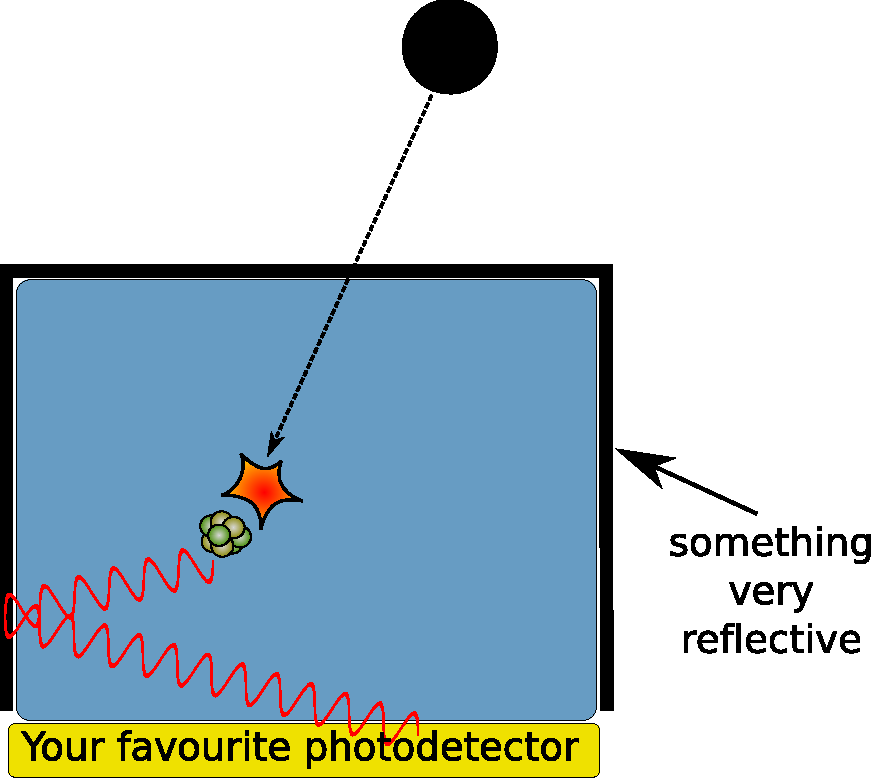
\includegraphics[width=0.6\linewidth]{SolidScintillator}}
  \end{textblock}

  \begin{textblock}{40}(80,80)
    \only<1>{\footnotesize(and/or ionisation, phonons)}
  \end{textblock}

  \begin{textblock}{65}(32,32)
    \only<2>{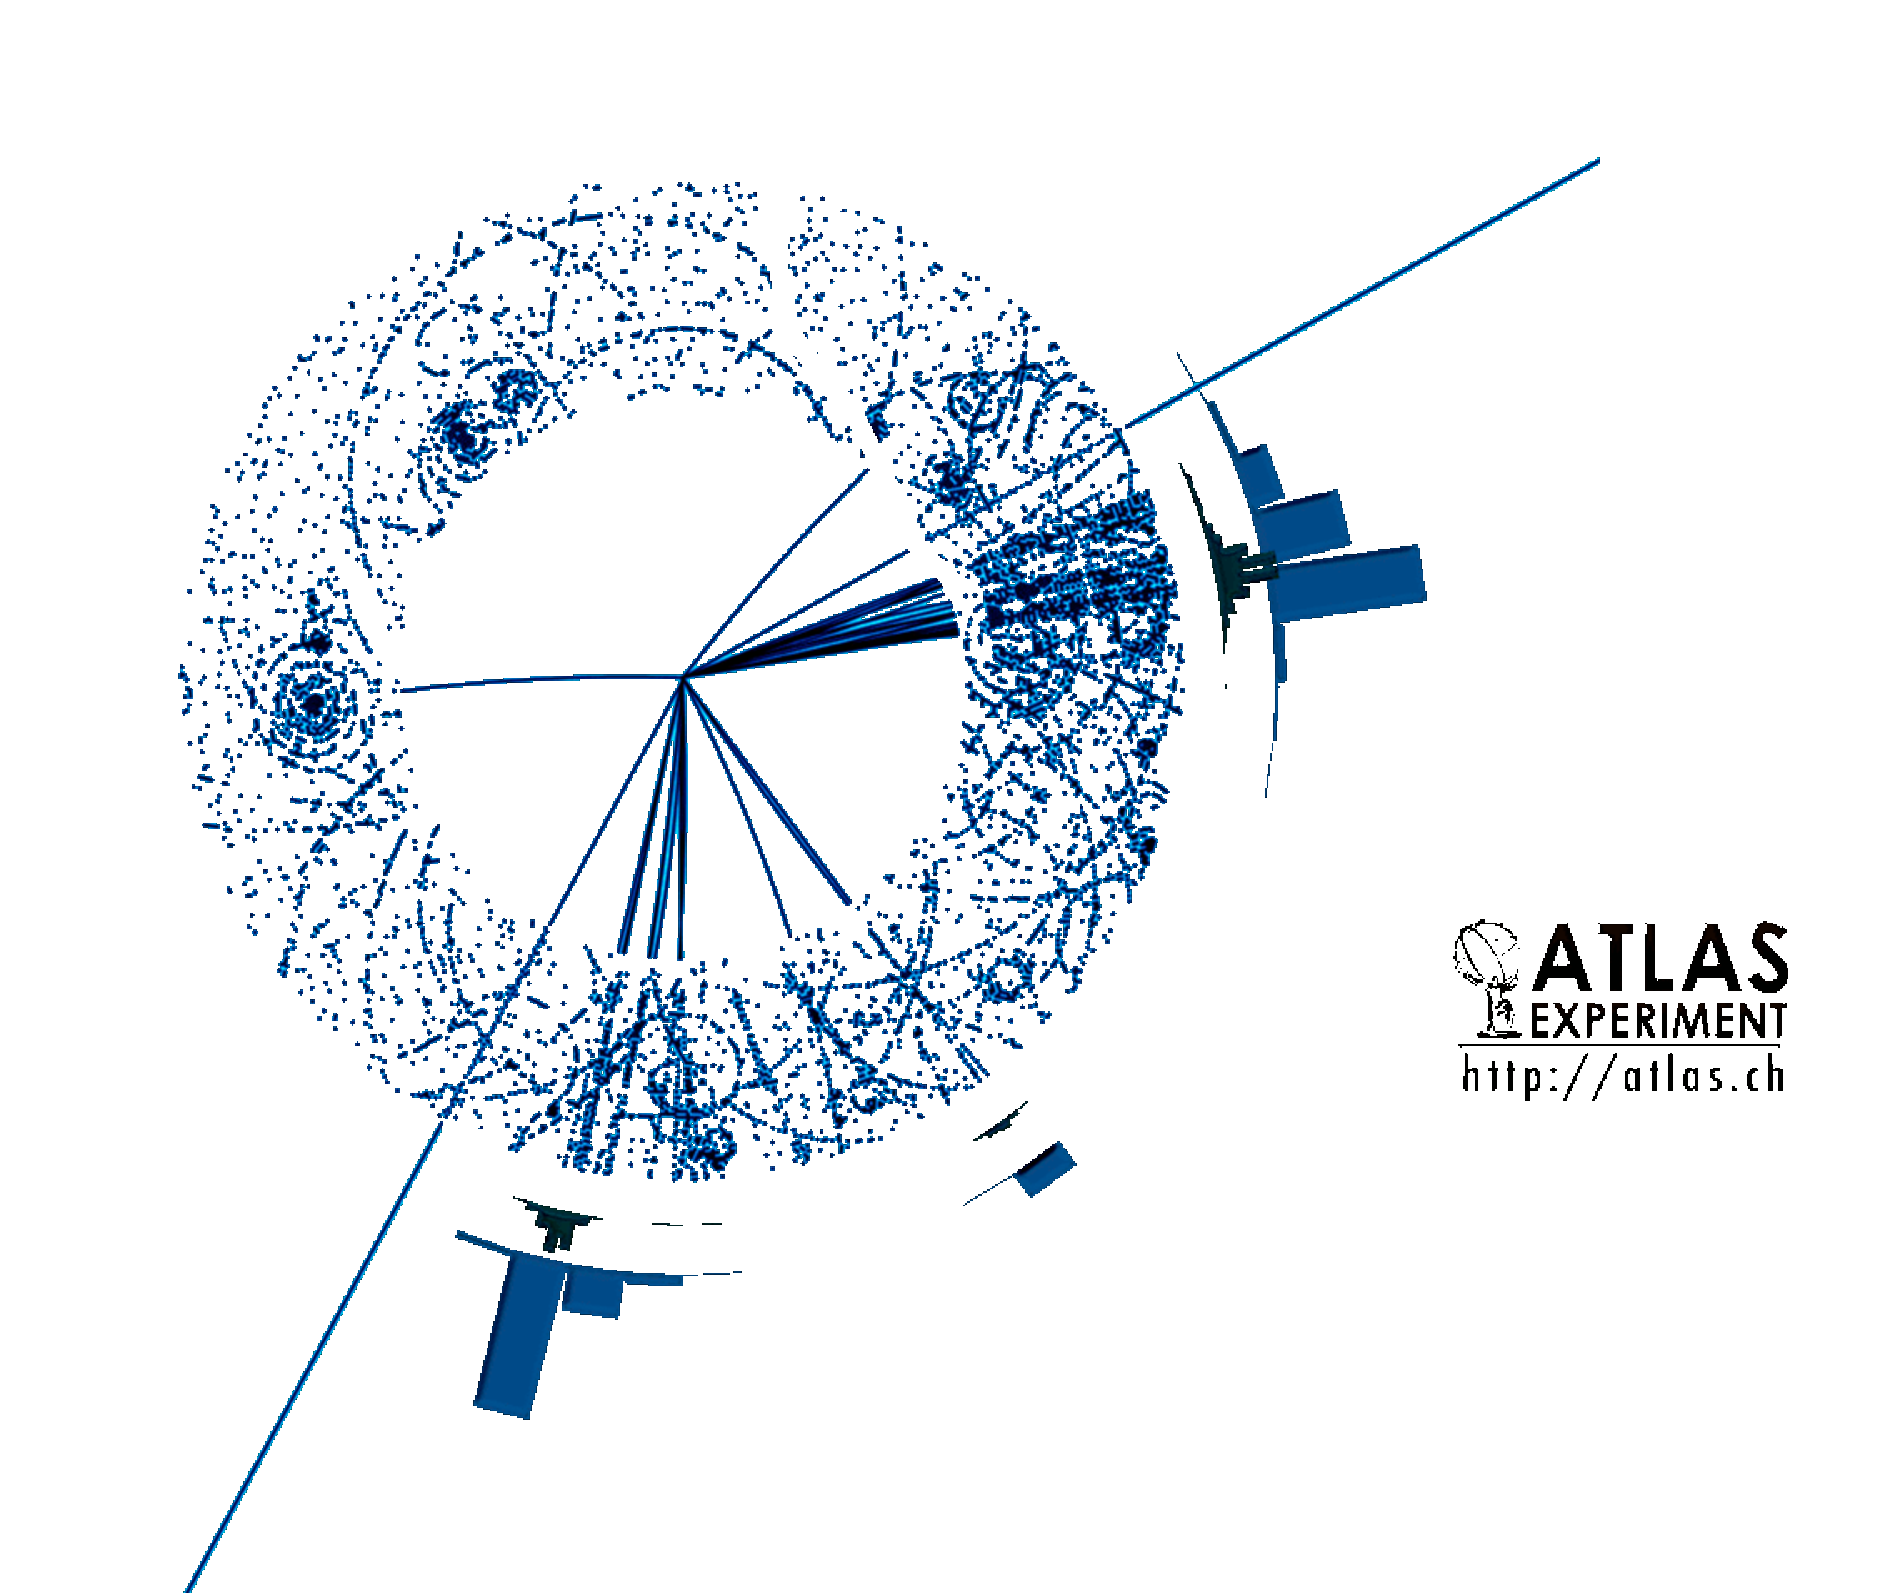
\includegraphics[width=\linewidth]{susy_sim3}}
  \end{textblock}

  \begin{textblock}{40}(75,44)
    \only<3->{\hspace{10mm}{\tiny(Weniger \textit{JCAP}, 1204.2797)}
    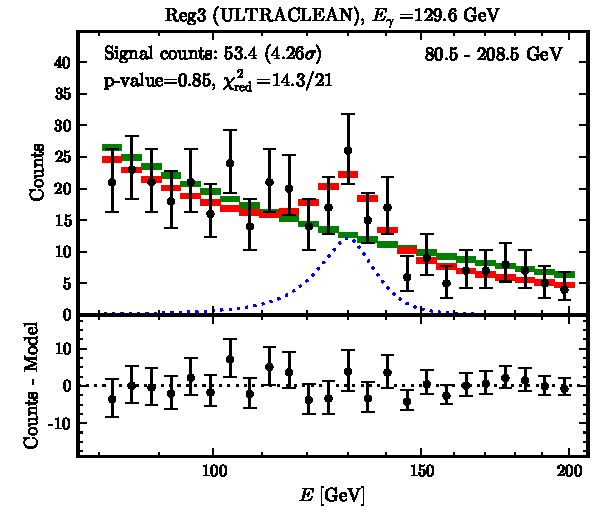
\includegraphics[width=\linewidth]{line}}
  \end{textblock}

\end{frame}


\subsection{Global fits}

\begin{frame}
\frametitle{BSM Model Scanning}

  \alert{Goals:} 
  \begin{enumerate} 
    \item given a particular theory, determine which parameter combinations fit all experiments, and how well \visible<2->{\\\hspace{5.15cm}\cblue{$\implies$ parameter estimation}}
    \item given multiple theories, determine which fit the data better, and quantify how much better \visible<2->{\cblue{$\implies$ model comparison}}
  \end{enumerate} 

\end{frame}

\begin{frame}
\frametitle{Putting it all together: global fits}  

  \alert{Issue 1:} Combining fits to different experiments\\
  Relatively easy -- composite likelihood ($\mathcal{L}_1\times\mathcal{L}_2 \equiv \chi^2_1 + \chi^2_2$ for simplest $\mathcal{L}$)
  {\footnotesize\begin{itemize}
    \item{dark matter relic density from WMAP}
    \item{direct detection}
    \item{indirect detection}
    \item{LHC searches}
    \item{precision electroweak tests at LEP}
    \item{LEP limits on sparticle masses}
    \item{$B$-factory data (rare decays, $b\rightarrow s\gamma$)}
    \item{muon anomalous magnetic moment (``$g-2$'')}
  \end{itemize}}
  \vspace{2mm}

\end{frame}

\begin{frame}
\frametitle{Putting it all together: global fits}  

  \alert{Issue 2:} Including the effects of uncertainties in input data\\
  Easy -- treat them as \emph{nuisance parameters}\vspace{4mm}

  \alert{Issue 3:} Finding the points with the best likelihoods\\
  \cbluewhen{Tough -- MCMCs, nested sampling, genetic algorithms, etc}{<2>}\vspace{4mm}

  \alert{Issue 4:} Comparing theories\\
  \cbluewhen{Depends -- Bayesian model comparison, $p$ values\\
  \hspace{40mm}($TS$ distribution? $\longrightarrow$ coverage???)}{<2>} 

\end{frame}


\begin{frame}
\frametitle{The state of play}

\pgfsetcornersarced{\pgfpoint{2mm}{2mm}}

\begin{textblock}{25}(1.5,26)
  \tikz \fill[blue, very nearly transparent] (1,1) rectangle (4.2,2.5);
\end{textblock}

\begin{textblock}{25}(1.5,43)
  \tikz \fill[blue, very nearly transparent] (1,1) rectangle (4.2,2.5);
\end{textblock}

\begin{textblock}{25}(32,32)
  \begin{tikzpicture}[line width=1.6pt, color=darkblue]
    \draw<2-3,5-6>[-stealth] (0,0) to (1.6,0.8);
    \draw<2-3,5-6>[-stealth] (0,2) to (1.6,1.2);
  \end{tikzpicture}%
  \begin{tikzpicture}[line width=1.6pt, color=red]
    \draw<4>[-stealth] (0,0) to (1.6,0.8);
    \draw<4>[-stealth] (0,2) to (1.6,1.2);
  \end{tikzpicture}
\end{textblock}

\begin{textblock}{25}(48.5,26)
  \only<2-4,6>{\tikz \fill[blue, very nearly transparent] (1,1) rectangle (4.2,4.45);}
  \only<5>{\tikz \fill[red, very nearly transparent] (1,1) rectangle (4.2,4.45);}
\end{textblock}

\begin{textblock}{25}(79,41.3)
  \begin{tikzpicture}[line width=1.6pt, color=darkblue]
    \draw<3-5>[-stealth] (0,0) to (1.3,0);
  \end{tikzpicture}%
  \begin{tikzpicture}[line width=1.6pt, color=red]
    \draw<6>[-stealth] (0,0) to (1.3,0);
  \end{tikzpicture}
\end{textblock}

\begin{textblock}{25}(93,37)
  \only<3-5>{\tikz \fill[blue, very nearly transparent] (1,1) rectangle (3.5,2);}
  \only<6>{\tikz \fill[red, very nearly transparent] (1,1) rectangle (3.5,2);}
\end{textblock}

\begin{columns}[t]
\column{0.3\textwidth}
  \textbf{\corange{Yesterday}}
\column{0.1\textwidth}
\column{0.3\textwidth}
  \visible<2->{\centering \textbf{\corange{Today}}}
\column{0.1\textwidth}
\column{0.22\textwidth}
  \visible<3->{\textbf{\corange{Tomorrow}}}
\end{columns}\vspace{2mm}

\begin{columns}[c]
\column{0.3\textwidth}

  \cblue{Experimentalists:}\\
  {
    Toy models\\
    Real constraints
  }\vspace{4mm}

  \cblue{Theorists:}\\
  {
    Real models\\
    Toy constraints
  }

\column{0.1\textwidth}
\column{0.3\textwidth}

  \visible<2->{
  \centering
    Real models\\
    $+$\\
    Real constraints\\
    $=$\\
    Real model parameter space constraints
  }

\column{0.1\textwidth}
\column{0.22\textwidth}

  \visible<3->{Theory space constraints}

\end{columns}\vspace{2mm}

\begin{enumerate}
\visible<4->{\item \alert<4>{Detailed astroparticle likelihoods for arbitrary models}}
\visible<5->{\item \alert<5>{Which experiments can we trust?}}
\visible<5->{\item \alert<5>{Compute time, coverage and scanning}}
\visible<6->{\item \alert<6>{Systematisation: Parameter space $\rightarrow$ Theory space}}
\end{enumerate}

\end{frame}

\section{Statistical Challenges}

\subsection{Detailed astroparticle likelihoods}

\begin{frame}

  \frametitle{Two different approaches to including astro data in BSM scans}



  \begin{enumerate}

  \item{Just use the published limits on $\langle \sigma v\rangle$ (or $\sigma_\mathrm{SI,SD}$)}

    \begin{itemize}

    \item{Fast -- can cover large parameter spaces}

    \item{Not so accurate -- experimental limits are invariably based on theoretical assumptions, e.g. $b\bar b$ spectrum}

    \item{Full likelihood function almost never available}

    \end{itemize}

  \item\alert<2-3>{Use the data points directly in BSM scans} 

    \begin{itemize}

    \item{Slow -- requires full treatment of instrument profile for each point}

    \item{Accurate -- can test each point self-consistently}

    \item{Allows marginalisation over theoretical assumptions}

    \item{Allows construction of full multi-dimensional likelihood function}

    \end{itemize}

  \visible<3>{\item\alert{(indirect only: use just flux upper limits)}}

  \end{enumerate}

\end{frame}


\begin{frame}
\frametitle{Gamma-rays}

Gamma-ray annihilation searches have been added to the global fits: 
\vspace{3mm}

\begin{columns}[t]

\column{0.54\linewidth}
\only<1>{\cblue{\textit{Fermi}-LAT}}%
\only<2>{\cblue{HESS}}

{\footnotesize
\only<1>{Satellite pair conversion telescope}%
\only<2>{Air \v{C}erenkov telescope}

\only<1>{Dwarf galaxy Segue 1}%
\only<2>{Milky Way$+$Carina$+$Sculptor$+$Sag dwarf}
}%
\vspace{2mm}

\only<1>{\tiny (PS, Conrad et al {\it JCAP}, 0909.3300)}%
\only<2>{\tiny(Ripken, Conrad \& PS {\it JCAP}, 1012.3939)}\vspace{2mm}

\only<1>{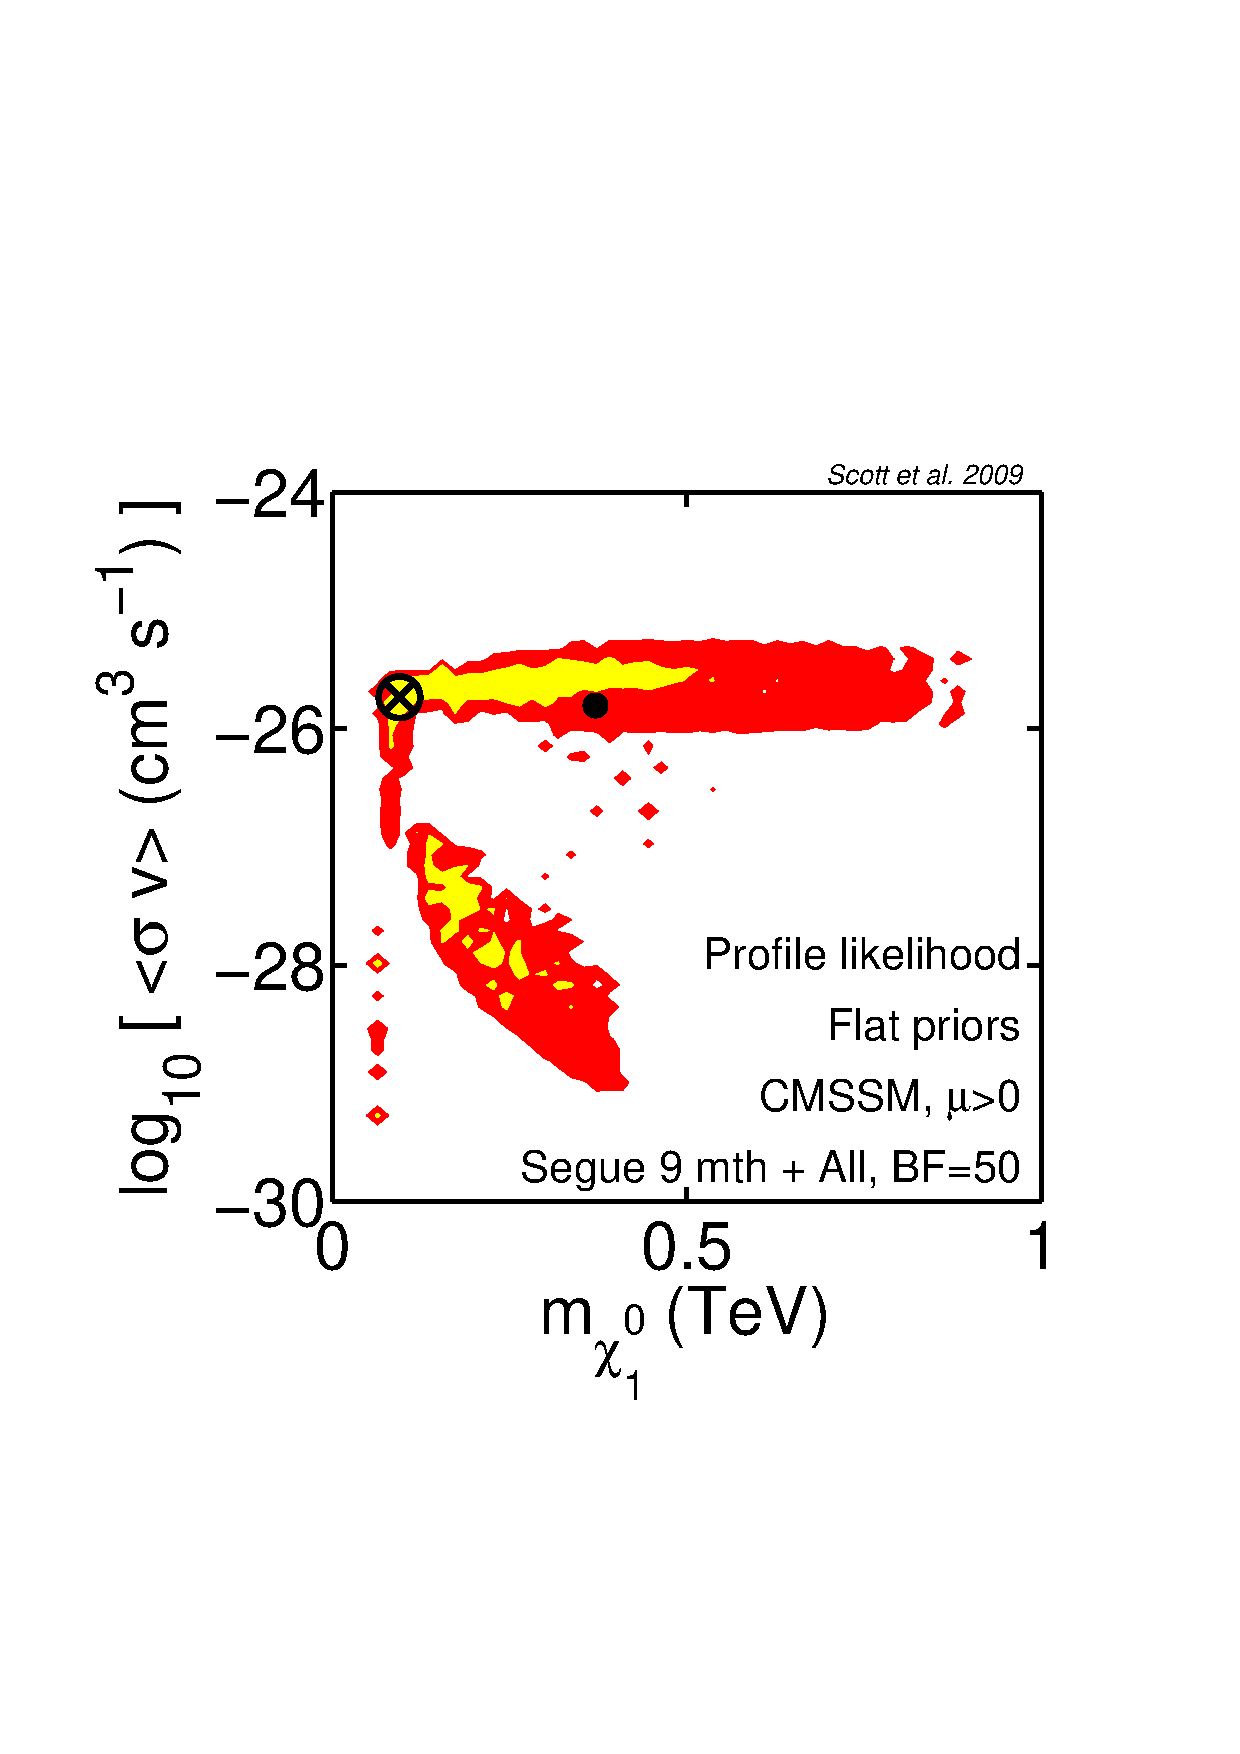
\includegraphics[height=0.6\textwidth, trim = 20 182 20 220, clip=true]{B50_H0_All_P_lin_2D_profl_7}}%
\only<2>{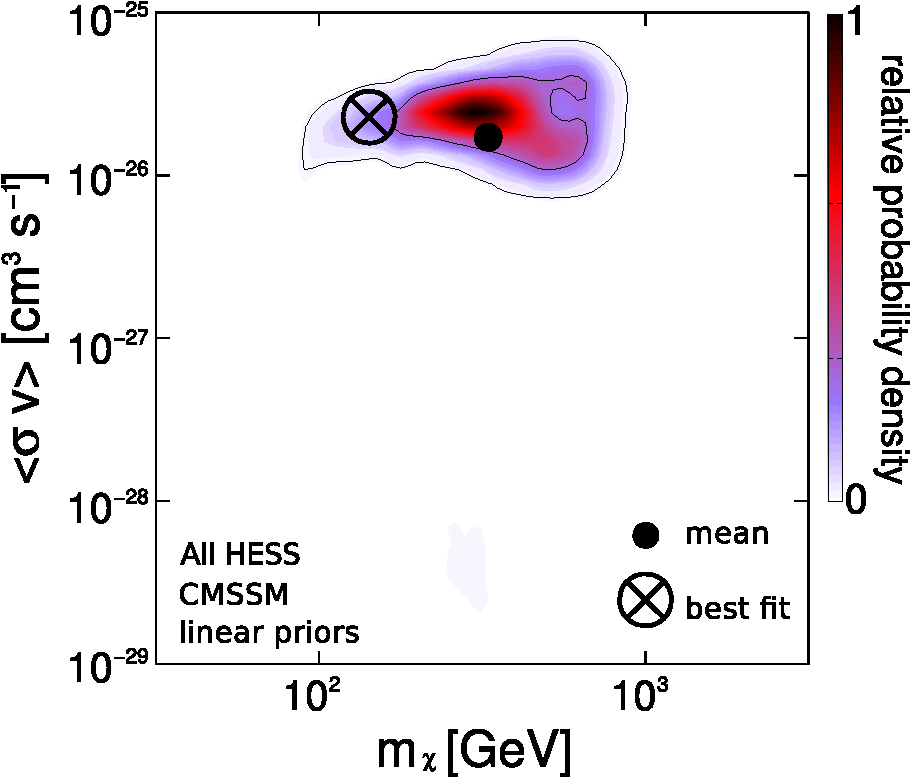
\includegraphics[height=0.6\textwidth]{allHESS}}

\column{0.6\linewidth}
\only<1>{\footnotesize\vspace{-3mm}
\begin{itemize}
\item Full binned Poissonian likelihood (no $\chi^2$ approximation)
\item Full treatment of PSF \textit{and} energy dispersion (with fast convolution library FLATlib) 
\item Marginalisation over systematic error on effective area
\item Diffuse BG from Fermi-LAT Galprop fits
\item Isotropic BG best-fit isotropic power law
\item $J$-factor from Martinez et al (\textit{JCAP}, 0902.4715; best at the time)
\end{itemize}
}%
\only<2>{
\begin{itemize}
\item $\chi^2$-based analysis using public flux limits
\item `Milky Way' = halo just beyond GC (45--150\,pc)
\item Virtual internal bremsstrahlung from co-annihilation strip models caught at high-$E$ by HESS 
\item but: $J$-factors for Sag dwarf rather uncertain

\end{itemize}
}

\end{columns}

\end{frame}

\begin{frame}

\frametitle{Advanced IceCube Likelihood}

\footnotesize
Full unbinned likelihood; number ($\Like_\mathrm{num}$), spectral ($\Like_\mathrm{spec}$) \& angular ($\Like_\mathrm{ang}$) parts:
\begin{equation}
\Like = \Like_\mathrm{num}(n|\theta_{\mathrm{signal+BG}})\prod_{i=1}^{n} \Like_{\mathrm{spec},i}\,\Like_{\mathrm{ang},i}
\end{equation}

\visible<1-3>{
  {\centering
  \only<1>{\cblue{\hspace{4mm}Mock signal reconstruction with IceCube-DeepCore (86-string)}\\}%
  \only<2->{Limits: \cblue{IceCube 22-string data} \hspace{5mm} vs. \hspace{5mm} \cblue{IceCube-DeepCore (86-string)}\\}%
  \only<1,2>{\centering\tiny(PS, Savage, Edsj\"o \& IceCube {\it JCAP}, 1207.0810)}%
  \only<3->{\tiny(PS, Savage, Edsj\"o \& IceCube {\it JCAP}, 1207.0810)\hspace{10mm}(Silverwood, PS, Danninger et al {\it JCAP}, 1210.0844)}%
  }
  \begin{columns}
  \column{0.58\linewidth}
    \only<2->{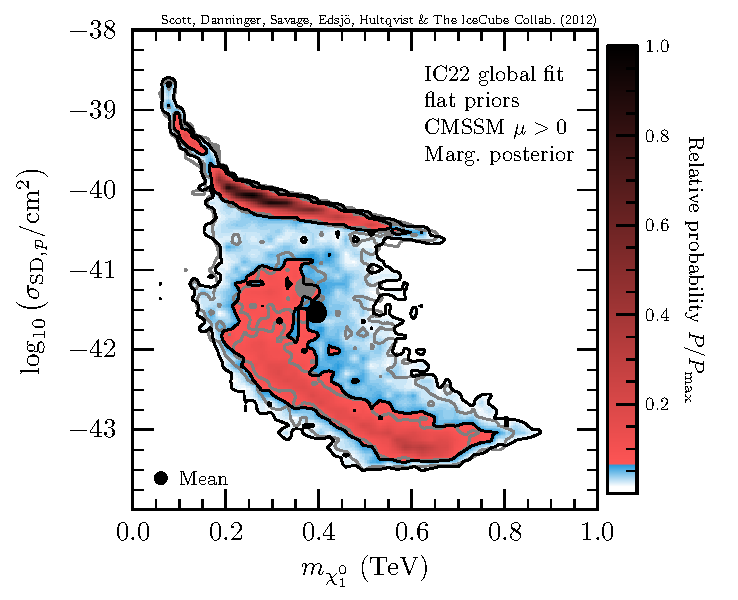
\includegraphics[width=0.85\textwidth]{IC22_marg3}}%
    \only<1>{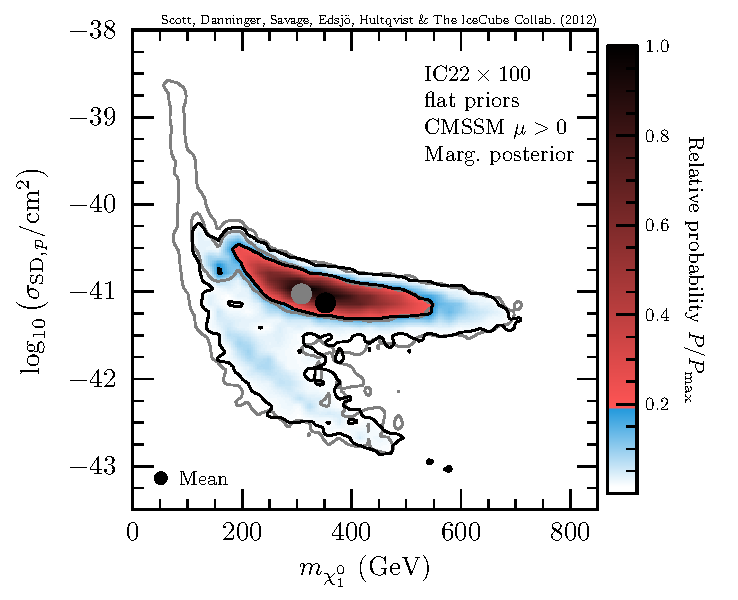
\includegraphics[width=0.85\textwidth]{recon2D_4}}
  \column{0.58\linewidth}
    \only<1>{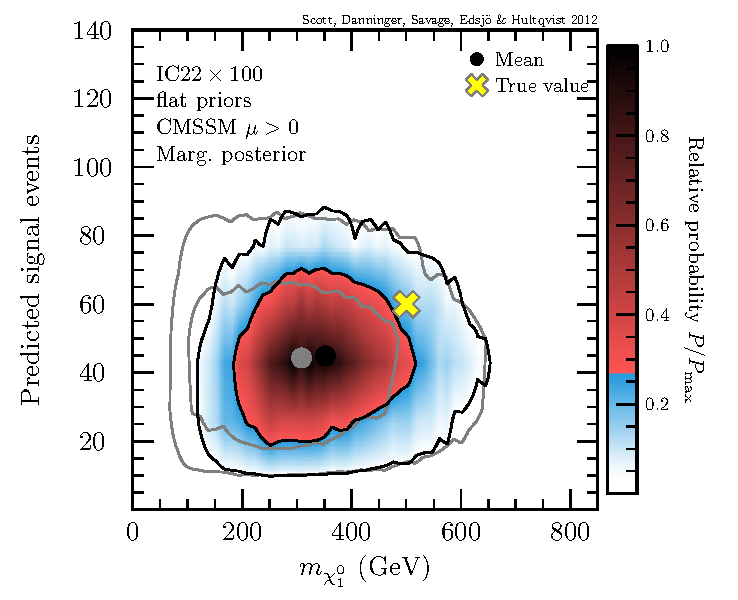
\includegraphics[width=0.85\textwidth]{recon2D_5}}%
    \only<2>{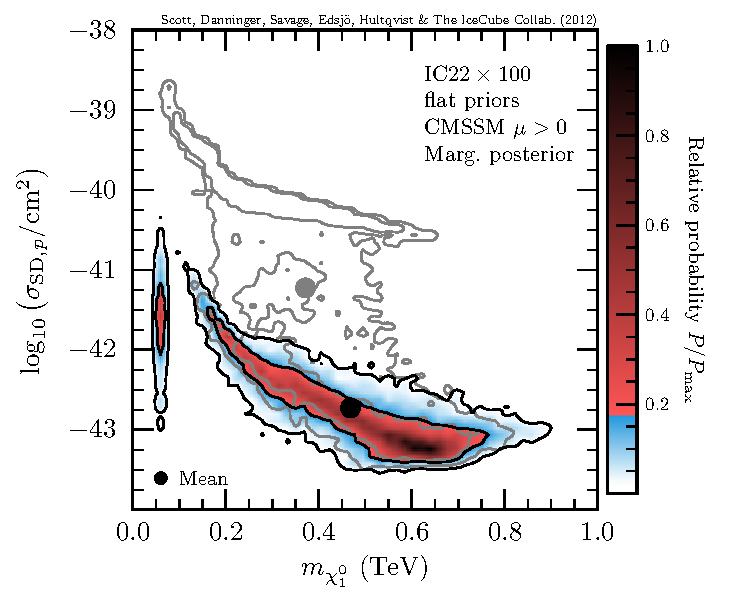
\includegraphics[width=0.85\textwidth]{IC22x100_marg3}}%
    \only<3->{\hspace{2mm}\tiny$\rightarrow$ IC86 has unique access to pts in more general MSSM\\
              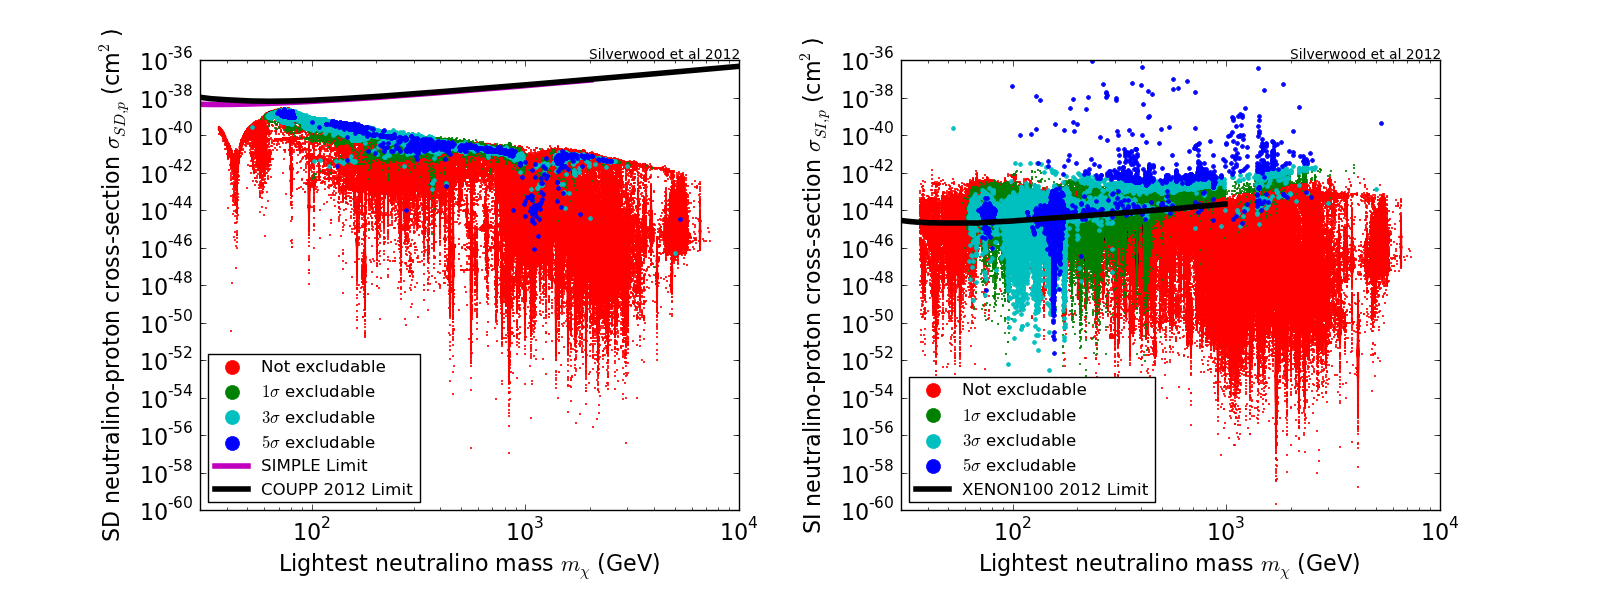
\includegraphics[width=0.9\textwidth, trim = 550 0 0 0, clip=true]{MSSM25}}
  \end{columns}
}

\only<4>{
\begin{textblock}{90}(15,39)
The examples here are CMSSM \& MSSM-25 -- but this about a framework, applicable to any model.  
\vspace{3mm}

{\alert{All methods are available implemented in DarkSUSY v5.0.6 and later: }{\color[rgb]{0.1, 0.0, 0.6}\href{www.darksusy.org}{www.darksusy.org}}
\vspace{3mm}}

{All IceCube data used are available at {\color[rgb]{0.1, 0.0, 0.6}\href{http://icecube.wisc.edu/science/data/ic22-solar-wimp}{http://icecube.wisc.edu/science/data/ic22-solar-wimp}} (and in DarkSUSY, for convenience)}\\
\end{textblock}
}

\end{frame}


\begin{frame}
\frametitle{Generalised DM CMB likelihood functions}

Simple CMB likelihood function, for
\begin{itemize}
\item Any combination of annihilation or decay channels
\item Any dark matter mass 
\item Any decay lifetime/annihilation cross-section
\end{itemize}
$\rightarrow$ just requires interpolating one number in a table.\vspace{5mm}

\visible<2-3>{
$f_\mathrm{eff}$ for annihilation:
\begin{equation}\footnotesize
 \ln\,\mathcal{L}(\langle\sigma v\rangle|m_\chi,r_i) = -\frac12 f_{\rm eff}^2(m_\chi,r_i) \lambda_1 c_1^2\,
 \left(\frac{\langle\sigma v\rangle}{2\times 10^{-27}{\rm cm}^3{\rm s}^{-1}}\right)^2\,\left(\frac{\rm GeV}{m_\chi}\right)^2
\label{loglike2}
\end{equation}
}

\visible<3>{
$\eta$ for decay:
\begin{equation}\footnotesize
\ln\, \mathcal{L}(\tau|m_\chi,r_i) = -\frac12\left(\delta\Omega\over\Omega_\mathrm{DM}\tau\right)^2\eta^2(\tau,m_\chi,r_i)
\end{equation}
}


\begin{textblock}{70}(15,48)
  \visible<4>{
    \begin{columns}
    \column{0.6\linewidth}
    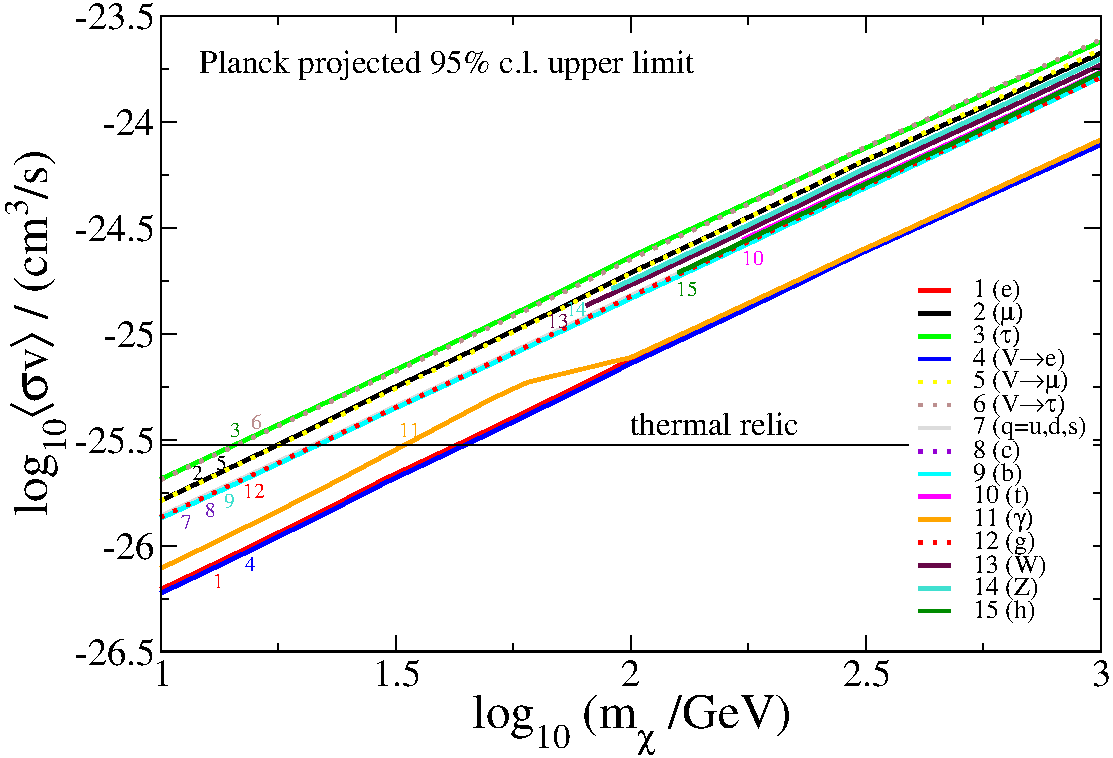
\includegraphics[width=1.1\textwidth]{planck-limit}
    \column{0.1\linewidth}
    \column{0.6\linewidth}
    \includegraphics[width=1.1\textwidth]{electrons-w-planck}
    \end{columns}
  }
\end{textblock}

\begin{textblock}{80}(15,49)
  \visible<1>{
  Cline \& PS, {\it JCAP}, 1301.5908, using
  \begin{itemize}
    \item CMB energy deposition from Slatyer, 1211.0283 and Finkbeiner et al, 1109.6322
    \item PYTHIA annihilation/decay spectra of Cirelli et al, 1012.4515.
  \end{itemize}
  }
\end{textblock}

\end{frame}

\begin{frame}

\frametitle{Direct detection likelihoods}

Much solid work done in implementing detailed direct detection likelihoods in pheno analyses -- \alert{details coming up this afternoon}
\\\vspace{3mm}
\tiny{Akrami, Savage et al 1011.4318, 1011.4297\\
Pato et al 1012.3458, 1106.0743, 1211.7063\\
Arina et al 1105.5121, 1210.4011\\
Strege et al 1107.1715, 1112.4192, 1201.3631, 1212.2636}

\begin{columns}
\column{0.5\textwidth}
    \tiny Pato et al 1211.7063
    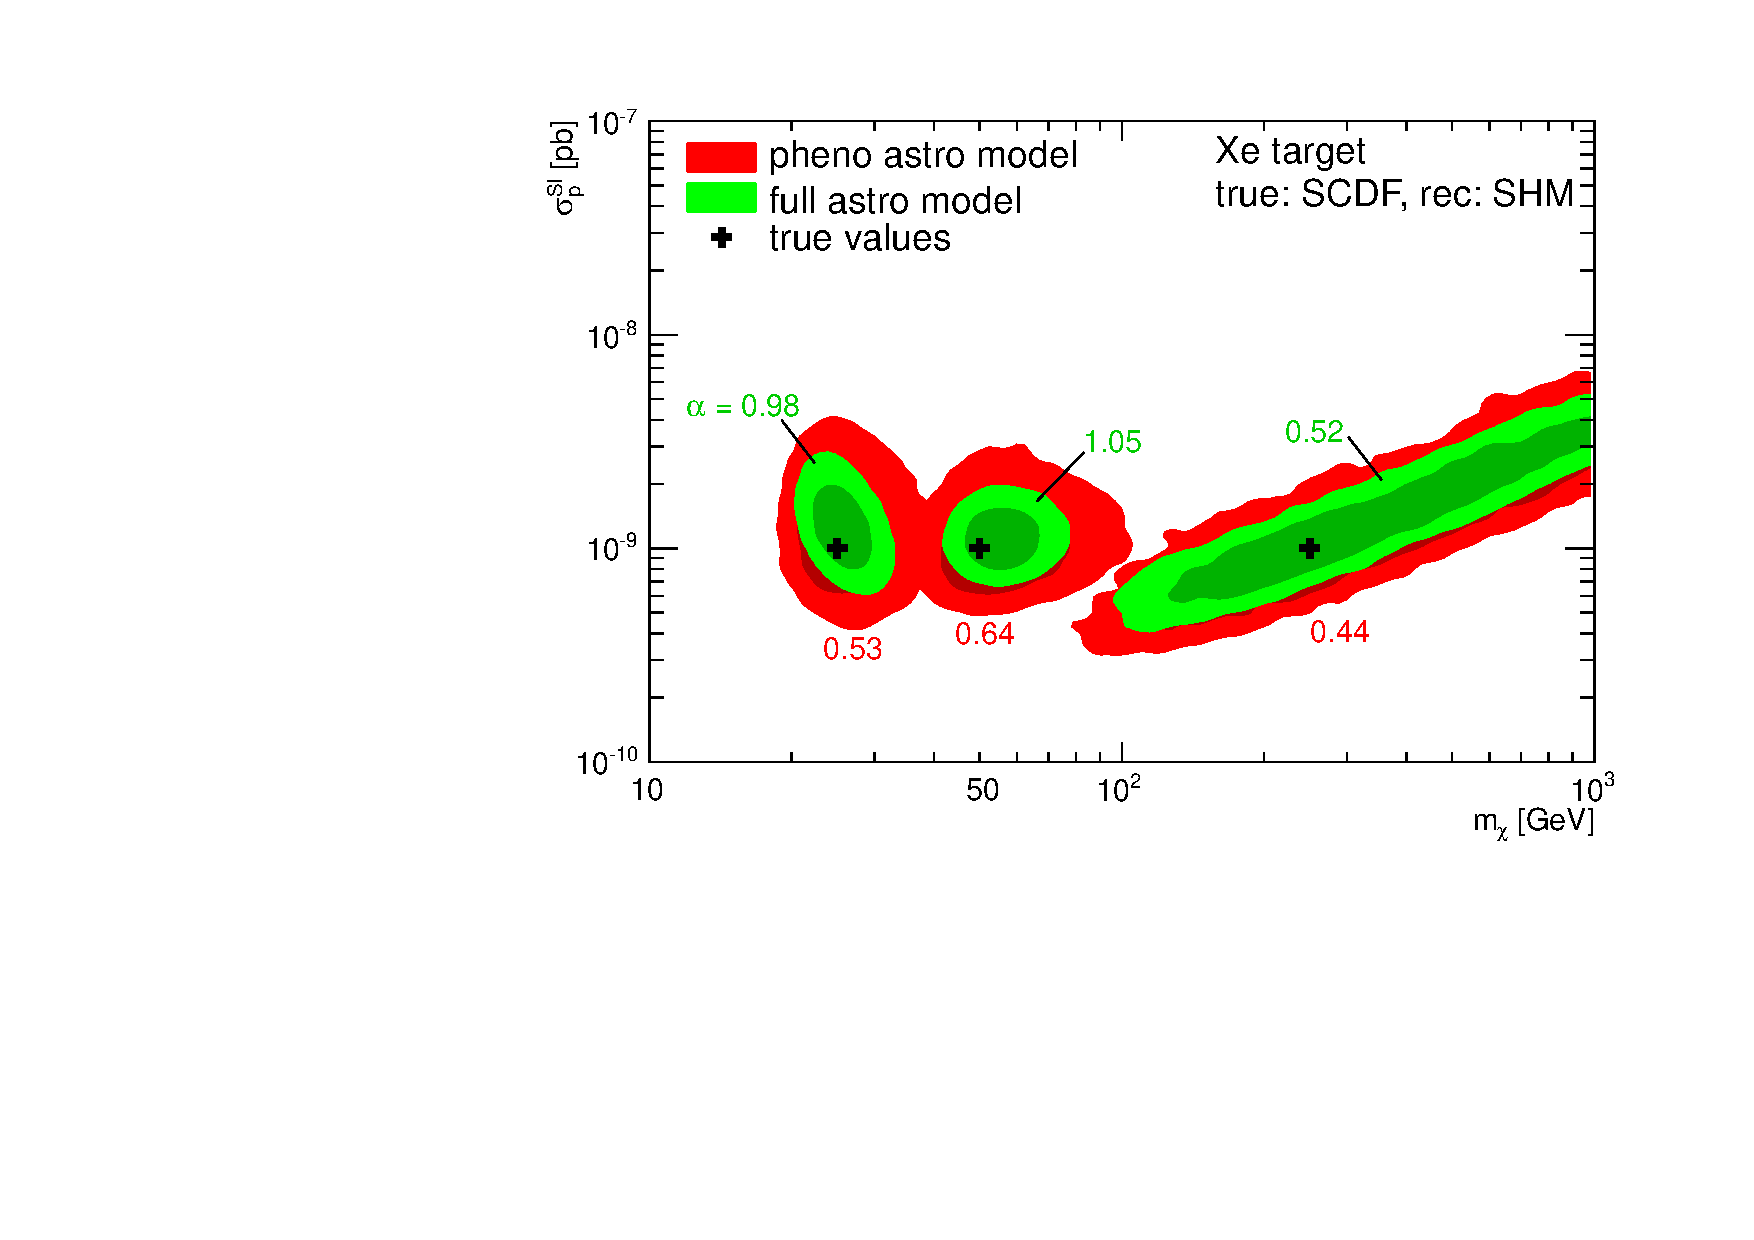
\includegraphics[width=\linewidth]{fig4a_phenofull}
\column{0.5\textwidth}
    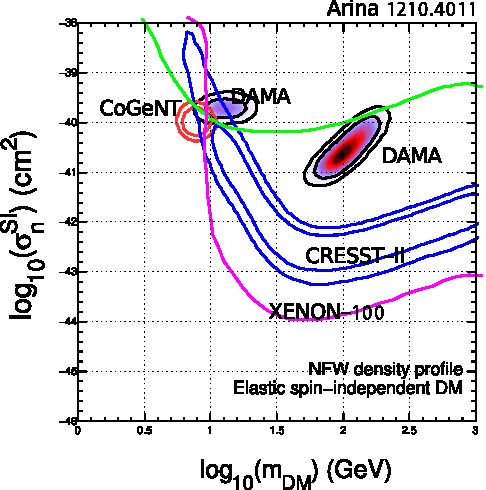
\includegraphics[width=0.8\linewidth]{arina_ex}
\end{columns}

\end{frame}

\subsection{Which experiments can we trust?}

\begin{frame}
\frametitle{Conflicting experimental results}
In many cases we have apparently inconsistent experimental results: anomalies, claimed detections, deviations, etc\vspace{5mm}

\begin{textblock}{100}(10,35)
  \visible<2>{%
    \textbf{Direct Detection}\\
    DAMA vs. CoGeNT vs. CRESST-II vs. Exclusions\\\vspace{2mm}
    \centering
    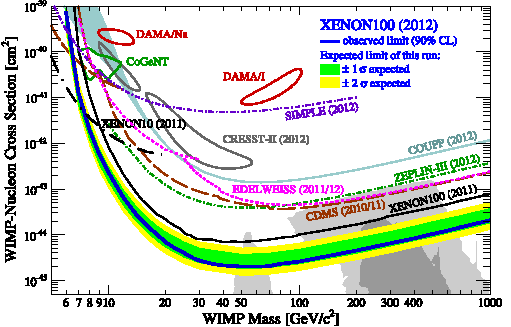
\includegraphics[width=0.63\linewidth]{XENON100_2012}
  }%
\end{textblock}

\begin{textblock}{100}(10,35)
  \visible<3>{%
    \textbf{Gamma-ray lines}\\
    130\,GeV line - to bump or not to bump\\\vspace{2mm}
    \begin{columns}
    \column{0.42\textwidth}
      \centering
      {\tiny(Weniger \textit{JCAP}, 1204.2797)}
      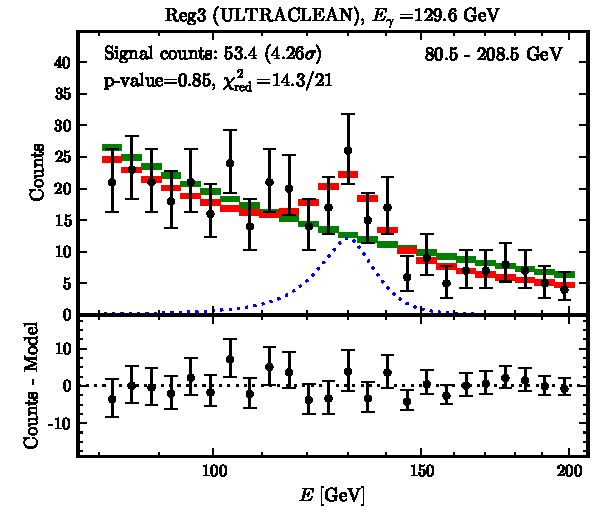
\includegraphics[width=\linewidth]{line}
    \column{0.6\textwidth}
      \includegraphics[width=\linewidth]{FermiLine2DEDisp}
    \end{columns}
  }%
\end{textblock}

\visible<4->{%
What do we do with the suspect data?%
\begin{enumerate}
\visible<5->{\item Keep it (remember to hold your nose)}
\visible<6->{\item Toss it out}
\visible<7->{\item Inflate the systematic errors}
\visible<8->{\item Give it some arbitrary down-weighting (prior)}
\visible<9->{\item Try to do something a bit more objective ($\rightarrow$ David's talk)}
\end{enumerate}\vspace{15mm}

}

\end{frame}

\subsection{Compute time, coverage and scanning}

\begin{frame}
\frametitle{Compute time example: The LHC likelihood monster}

\visible<1->{
\begin{exampleblock}{Time per point:}
$\mathcal{O}(minute)$ in \alert{best} cases
\end{exampleblock}
}

\visible<2->{
\begin{exampleblock}{Time per point for global fits to converge:}
$\mathcal{O}(seconds)$ in \alert{worst} cases
\end{exampleblock}
}

\visible<3->{
\begin{exampleblock}{Challenge:}
About 2 orders of magnitude too slow to actually include LHC data in global fits properly
\end{exampleblock}
}

\end{frame}

\begin{frame}
\frametitle{Taming the LHC monster}

\only<1,2>{
\begin{exampleblock}{First Order Response:}
``Test if things depend on the other parameters (hope not), re-simulate published exclusion curve''
\end{exampleblock}

\visible<2>{
\vspace{5mm}
Not that great, but OK in some cases
\begin{itemize}    
  \item At least have some sort of likelihood this time
  \item Still a bit screwed if things do depend a lot on other parameters, but
  \item allows (potentially shaky) extrapolation, also to non-CMSSM models
\end{itemize}

\vspace{5mm}
Fittino, Mastercode
}}

\only<3,4>{
\begin{exampleblock}{Second Order Response:}
``That's ridiculous.  I've never met a calculation I can't speed up.  There must be some way to have my cake and eat it too''
\end{exampleblock}

\visible<4>{
\vspace{5mm}
Maybe -- this is the challenge.
\begin{itemize}    
  \item Interpolated likelihoods (how to choose nodes?)
  \item Neural network functional approximation (how to train accurately?)
  \item Some sort of smart reduction based on event topology? 
  \item Something else?
\end{itemize}
}}

\end{frame}

\begin{frame}
\frametitle{Coverage}
\cblue{We don't \textit{*really*} know the distribution of our test statistic in BSM global fits, as it is too expensive to Monte Carlo}

      \begin{itemize}\footnotesize
                 \item coverage is rarely spot-on unless mapping from parameters to data-space is linear \\
                 {\tiny(Akrami, Savage, PS et al {\it JCAP}, 1011.4297, Bridges et al {\it JHEP}, 1011.4306, Strege et al {\it PRD}, 1201.3631)}
                 \item $p$-value assessments of goodness of fit should be viewed with scepticism ($\rightarrow$MasterCode)
                 \end{itemize}

\visible<2>{\cblue{What do we do for a CL/$p$-value when we can't obtain the distribution of our test statistic??}}

\end{frame}

\begin{frame}
\frametitle{Scanning and Convergence}
\cblue{Convergence remains an issue, especially for profile likelihood}\vspace{2mm}

Messy likelihood $\implies$ best-fit point can be (and often is) easily missed {\tiny(Akrami, PS et al {\it JHEP}, 0910.3950, Feroz et al {\it JHEP}, 1101.3296)}
      \begin{itemize}\footnotesize
                 \item frequentist CLs are often off, as isolikelihood levels are chosen incorrectly
                 \item can impact coverage (overcoverage, or masking of undercoverage due to non-$\chi^2$ $TS$ distribution)
                 \item need to use multiple priors and scanning algorithms (one optimised for profile likelihoods?)  
                 \end{itemize}
\visible<2>{
  \vspace{-2mm}
  \begin{columns}
  \column{0.35\textwidth}
    \footnotesize
      $\rightarrow$ Differential Evolution\\\hspace{4mm}may help\\\vspace{2mm}
    DEIS algorithm (\alert{D}ifferential \alert{E}volution with \alert{I}mportance \alert{S}ampling)\\\vspace{1mm}
    \tiny{Roebber, PS, Putze \& Holder, in prep}
  \column{0.35\textwidth}
    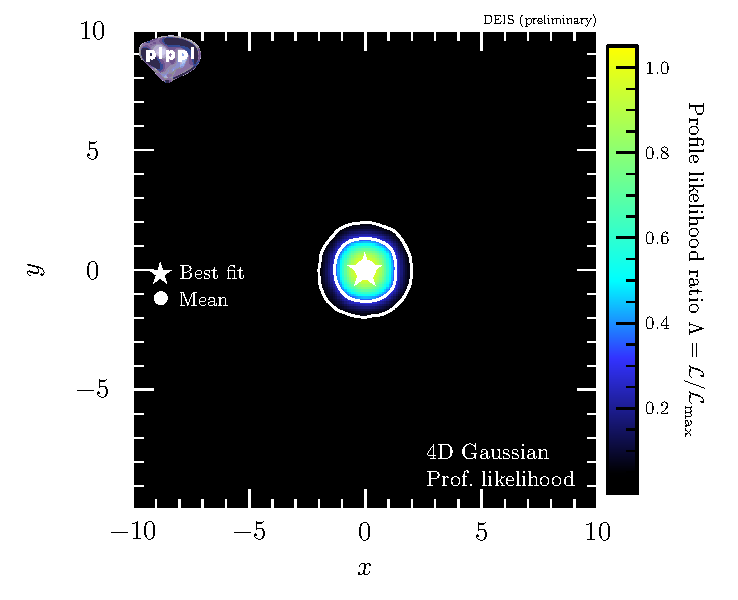
\includegraphics[width=\textwidth]{example_4_5_like2D}
  \column{0.35\textwidth}
    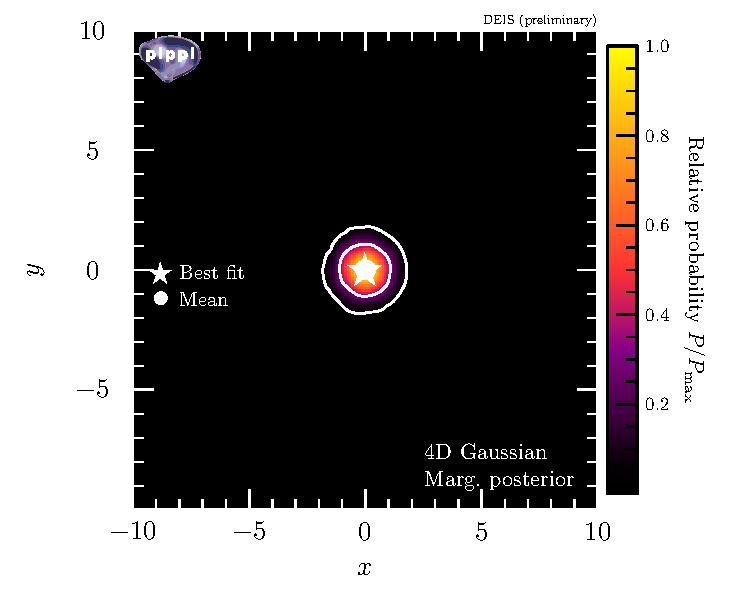
\includegraphics[width=\textwidth]{example_4_5_post2D}
  \end{columns}
}

\end{frame}


\subsection{Systematisation: Parameter space $\rightarrow$ Theory space}

\begin{frame}
\frametitle{CMSSM, SMS $\ne$ BSM}

(SMS = Simplified Model Spectrum)
\vspace{3mm}

Want to do model comparison to actually work out which theory is right\ldots
\vspace{3mm}

\begin{exampleblock}{Challenge:}
How do I easily adapt a global fit to different BSM theories?
\end{exampleblock}

\visible<2>{
Somehow, we must recast things quickly to a new theory 
\begin{itemize}
\item data
\item likelihood functions
\item scanning code `housekeeping'
\item even predictions
\end{itemize}
$\implies$ a new, very abstract global fitting framework
}

\end{frame}

\begin{frame}
\frametitle{Hitting the wall}

Issues with current global fit codes:
\begin{itemize}
\item Strongly wedded to a few theories (e.g. constrained MSSM / mSUGRA)
\item Strongly wedded to a few theory calculators
\item All datasets and observables basically hardcoded
\item Rough or non-existent treatment of most experiments (astroparticle + collider especially)
\item Sub-optimal statistical methods / search algorithms
\item $\implies$ \textit{already hitting the wall on theories, data \& computational methods}
\end{itemize}

\end{frame}

\begin{frame}
\frametitle{Closing remarks}

\begin{itemize}
\item{Robust analysis of astroparticle data in the context of new physics requires multi-messenger global fits}
\item{\visible<2->{Detailed astroparticle likelihoods for BSM searches are progressing well}}
\item{\visible<3->{Our decision-making process for including/excluding datasets needs improvement}}
\item{\visible<4->{Coverage, scanning and general compute time all mess with each other -- some progress, but more work needed}}
\item{\visible<5->{The move to theory space has begun -- but requires all the rest to be solved too!}}
\end{itemize}


\end{frame}

\end{document}




